%% Supplementary Information — leakage-controlled cautionary study
\documentclass{article}
\usepackage[utf8]{inputenc}
\usepackage[margin=1in]{geometry}
\usepackage{amsmath,amssymb}
\usepackage{graphicx}
\usepackage{booktabs}
\usepackage{multirow}
\usepackage[numbers]{natbib}
\usepackage{hyperref}
\usepackage{url}
\providecommand{\bibcommenthead}{}% no-op: emitted by sn bst, undefined in article class
\providecommand{\botrule}{\bottomrule}% sn-jnl macro, map to booktabs in article class
\providecommand{\yes}{yes}\providecommand{\no}{no}% factorial-table marks (undefined in article class)

\title{Supplementary Information:\\ A Leakage-Controlled Evaluation Protocol for Data Selection in DP Federated Anomaly Detection for IIoT}
\author{}\date{}

\begin{document}
\maketitle

All numbers are computed from the released result files; each table cites its source.
No value is hand-entered. Unless noted, results use a reconstruction autoencoder trained
on normal-operation data only and end-to-end $(\varepsilon,\delta)$ DP calibration.
Seed counts are stated per table.

\section{Full selection-comparison table}\label{supp:char}
Table~\ref{tab:scharfull} gives the complete version of the main paper's
selection-invariance result: full normal data versus three matched-size selection rules,
for every dataset and budget (\texttt{characterization.json}). The cross-mode differences
are within seed noise on SKAB and TEP; on SWaT they are larger but never favour a learned
rule over random or full.

\begin{table}[h]\centering
\caption{Selection has no advantage. F1 (mean$\pm$std, $10$ seeds, centralised DP,
normal-only training). Source: \texttt{characterization.json}}\label{tab:scharfull}
\begin{tabular}{@{}llcccc@{}}
\toprule
Dataset & $\varepsilon$ & full & random & temporal & diversity \\
\midrule
\multirow{4}{*}{SKAB}
 & 0.5 & 0.210$\pm$0.004 & 0.207$\pm$0.002 & 0.207$\pm$0.002 & 0.207$\pm$0.004 \\
 & 1.0 & 0.213$\pm$0.012 & 0.208$\pm$0.004 & 0.209$\pm$0.004 & 0.208$\pm$0.004 \\
 & 2.0 & 0.214$\pm$0.013 & 0.210$\pm$0.006 & 0.212$\pm$0.007 & 0.209$\pm$0.009 \\
 & 4.0 & 0.214$\pm$0.013 & 0.211$\pm$0.009 & 0.211$\pm$0.011 & 0.212$\pm$0.010 \\
\midrule
\multirow{4}{*}{SWaT}
 & 0.5 & 0.366$\pm$0.017 & 0.329$\pm$0.008 & 0.317$\pm$0.002 & 0.315$\pm$0.003 \\
 & 1.0 & 0.325$\pm$0.049 & 0.350$\pm$0.016 & 0.324$\pm$0.004 & 0.321$\pm$0.004 \\
 & 2.0 & 0.321$\pm$0.042 & 0.361$\pm$0.021 & 0.326$\pm$0.006 & 0.325$\pm$0.005 \\
 & 4.0 & 0.325$\pm$0.037 & 0.337$\pm$0.040 & 0.303$\pm$0.024 & 0.304$\pm$0.029 \\
\midrule
\multirow{4}{*}{TEP}
 & 0.5 & 0.444$\pm$0.000 & 0.444$\pm$0.000 & 0.444$\pm$0.000 & 0.444$\pm$0.000 \\
 & 1.0 & 0.444$\pm$0.000 & 0.444$\pm$0.000 & 0.444$\pm$0.000 & 0.444$\pm$0.000 \\
 & 2.0 & 0.444$\pm$0.000 & 0.444$\pm$0.000 & 0.444$\pm$0.000 & 0.444$\pm$0.000 \\
 & 4.0 & 0.444$\pm$0.000 & 0.444$\pm$0.000 & 0.444$\pm$0.000 & 0.444$\pm$0.000 \\
\botrule
\end{tabular}
\end{table}

\paragraph{TEP saturation.} On TEP the percentile-thresholded reconstruction detector
attains precision $\approx1.0$ and recall $\approx0.29$ for a deterministic F1 $=0.444$;
the ranking is invariant to DP noise. TEP therefore serves only as a $\rho\!\approx\!1$
control where, correctly, no redundancy exists to remove.

\section{High-signal regime (strong detector)}\label{supp:strong}
To check that the null is not a floor effect, we train the reconstruction detector
for $40$ epochs (normal-only), reaching a genuine high-signal regime, and repeat the
selection comparison under DP. Table~\ref{tab:sstrong} gives the full point-wise and
point-adjusted F1. No learned rule (temporal, diversity) beats random or full beyond
one standard deviation in any cell, consistent with the recent (preprint) suppression
result of Miranda-Pascual et al.~\cite{stoddard2026suppress}. Point-adjusted F1 is shown only
for comparability with the strong-detector literature and is known to inflate
scores~\cite{kim2022rigorous}; the point-wise column is the appropriate metric.

\begin{table}[h]\centering
\caption{High-signal regime, $40$-epoch detector. F1 (mean$\pm$std, $10$ seeds, DP).
Source: \texttt{strong\_selection.json}}\label{tab:sstrong}
\begin{tabular}{@{}lllcccc@{}}
\toprule
Dataset & metric & $\varepsilon$ & full & random & temporal & diversity \\
\midrule
\multirow{4}{*}{SWaT} & \multirow{2}{*}{pt-wise} & 0.5 & 0.335$\pm$0.036 & 0.357$\pm$0.018 & 0.321$\pm$0.004 & 0.319$\pm$0.003 \\
 & & 2.0 & 0.321$\pm$0.028 & 0.324$\pm$0.049 & 0.226$\pm$0.030 & 0.236$\pm$0.039 \\
 & \multirow{2}{*}{pt-adj} & 0.5 & 0.651$\pm$0.010 & 0.657$\pm$0.005 & 0.648$\pm$0.001 & 0.647$\pm$0.001 \\
 & & 2.0 & 0.648$\pm$0.007 & 0.649$\pm$0.013 & 0.624$\pm$0.007 & 0.626$\pm$0.010 \\
\midrule
\multirow{4}{*}{SKAB} & \multirow{2}{*}{pt-wise} & 0.5 & 0.212$\pm$0.010 & 0.208$\pm$0.002 & 0.210$\pm$0.002 & 0.209$\pm$0.003 \\
 & & 2.0 & 0.216$\pm$0.010 & 0.214$\pm$0.011 & 0.216$\pm$0.010 & 0.216$\pm$0.012 \\
 & \multirow{2}{*}{pt-adj} & 0.5 & 0.700$\pm$0.026 & 0.768$\pm$0.007 & 0.762$\pm$0.021 & 0.756$\pm$0.026 \\
 & & 2.0 & 0.696$\pm$0.029 & 0.693$\pm$0.030 & 0.697$\pm$0.024 & 0.696$\pm$0.024 \\
\botrule
\end{tabular}
\end{table}

\section{Artifact audit (federated, corrected SIL fit)}\label{supp:artifact}
\paragraph{The original (protocol-violating) numbers.} For transparency, Table~\ref{tab:naive}
gives the per-cell SWaT result from the protocol-violating pipeline that motivated the case study: the
$3\sigma$ gate fit on full private (anomaly-containing) data and the detector trained on the
contaminated set. This is the source of the $+0.05$ to $+0.16$ F1 ``advantage'' quoted in the
main text (\texttt{paper\_results.json}); it is reproduced from the released artifact, not the leakage-controlled pipeline, and is shown only to document the failure mode.

\begin{table}[h]\centering
\caption{Protocol-violating pipeline, SWaT. F1 (mean). The spurious advantage that
the protocol removes. Source: \texttt{paper\_results.json}}\label{tab:naive}
\begin{tabular}{@{}lcccc@{}}
\toprule
Method & $\varepsilon{=}0.5$ & $\varepsilon{=}1$ & $\varepsilon{=}2$ & $\varepsilon{=}4$ \\
\midrule
dedup (uncontrolled)    & 0.273 & 0.301 & 0.333 & 0.352 \\
no-dedup (uncontrolled)    & 0.219 & 0.203 & 0.201 & 0.196 \\
\midrule
spurious gain    & $+0.054$ & $+0.098$ & $+0.132$ & $+0.156$ \\
\botrule
\end{tabular}
\end{table}

Table~\ref{tab:honest} shows the SWaT comparison under the leakage-controlled fix (the
$3\sigma$ preservation gate fit on public normal-only data instead of full private data).
The large advantage seen with the original (private+anomaly) fit disappears: training with
deduplication ties or loses to same-budget DP-FL without it in $6$ of $8$ SWaT cells
(\texttt{honest\_rerun.json}); the remaining cells are within seed noise and there is no
matched random arm here, so this is not evidence of a learned-rule benefit.

\begin{table}[h]\centering
\caption{SWaT, corrected (public-normal) gate. F1 (mean, $10$ seeds). Source:
\texttt{honest\_rerun.json}}\label{tab:honest}
\begin{tabular}{@{}llcccc@{}}
\toprule
Partition & Method & $\varepsilon{=}0.5$ & $\varepsilon{=}1$ & $\varepsilon{=}2$ & $\varepsilon{=}4$ \\
\midrule
\multirow{2}{*}{IID} & no-dedup & 0.221 & 0.219 & 0.220 & 0.185 \\
 & dedup & 0.229 & 0.206 & 0.210 & 0.180 \\
\midrule
\multirow{2}{*}{Dirichlet} & no-dedup & 0.231 & 0.219 & 0.174 & 0.198 \\
 & dedup & 0.218 & 0.211 & 0.196 & 0.182 \\
\botrule
\end{tabular}
\end{table}

\section{Which protocol rule kills the utility artifact?}\label{supp:ablation}
The protocol bundles two utility-side requirements: Rule~1 (selection statistics on
\emph{public} data) and Rule~2 (detector trained on \emph{normal-only} data).
Table~\ref{tab:ablation} decomposes the SWaT deduplication gain over the $2\times2$ of
these rules ($5$ seeds, IID partitions, \texttt{protocol\_ablation.json}). Three things
follow. First, the protocol-violating pipeline's gain ($+0.038\pm0.011$ and $+0.095\pm0.024$ at
$\varepsilon{=}0.5,2$) is removed by \emph{either} rule on its own: fixing Rule~1 alone
cuts it to $+0.011$/$+0.020$, and fixing Rule~2 alone to $-0.005$/$+0.045$ (the latter
within seed noise, std $0.062$). Second, once Rule~2 is applied the gate-reference
choice (Rule~1) has \emph{no further effect}---the leakage-controlled and ``fix Rule~2 only'' columns are identical to the digit---because the artifact requires the detector to
actually train on the anomaly-contaminated samples the gate preserves; remove that
(Rule~2) and the gate's choice is moot. Normal-only training is thus the load-bearing
requirement for the \emph{utility} artifact, with the public-gate rule reinforcing it
only under contaminated training. Third, we nonetheless keep Rule~1: it closes the
selection-statistics privacy leak ($\varepsilon_{\text{sel}}$) independently of utility,
and the fuller $10$-seed audit (Table~\ref{tab:honest}) confirms the gain is gone under
the complete protocol.

\begin{table}[h]\centering
\caption{Factorial ablation of the two utility rules. SWaT deduplication gain
$=$F1(dedup)$-$F1(no-dedup), mean$\pm$std over $5$ seeds. Source:
\texttt{protocol\_ablation.json}}\label{tab:ablation}
\begin{tabular}{@{}lcccc@{}}
\toprule
Config & R1 public gate & R2 normal-only & gain $\varepsilon{=}0.5$ & gain $\varepsilon{=}2$ \\
\midrule
uncontrolled     & \no & \no & $+0.038\pm0.011$ & $+0.095\pm0.024$ \\
fix R1 only      & \yes & \no & $+0.011\pm0.008$ & $+0.020\pm0.018$ \\
fix R2 only      & \no & \yes & $-0.005\pm0.011$ & $+0.045\pm0.062$ \\
controlled (R1+R2) & \yes & \yes & $-0.005\pm0.011$ & $+0.045\pm0.062$ \\
\botrule
\end{tabular}
\end{table}

\section{Membership inference: the evaluation-split artifact}\label{supp:mia}
We run two attacks: a \emph{weak} loss-threshold attack (rank probes by the target
detector's reconstruction loss; lower loss $\Rightarrow$ more likely member) and a
\emph{calibrated} LiRA-style attack. The headline question is not attack strength but the
member/non-member split.

\paragraph{Attack formulation.} For a target record $z$ and released detector $\theta$, let
$\ell(\theta,z)$ be the per-sample reconstruction loss. We train $N{=}8$ reference detectors
$\{\theta_j\}$ on random halves of an auxiliary pool; for record $z$ the references that did
\emph{not} see $z$ give an \emph{out} distribution
$\mathcal{N}(\mu_{\text{out}}(z),\sigma_{\text{out}}^2(z))$. The LiRA score is the one-sided
offline likelihood-ratio statistic
\[
\Lambda(z) \;=\; \frac{\mu_{\text{out}}(z)-\ell(\theta,z)}{\sigma_{\text{out}}(z)},
\]
i.e.\ how many standard deviations below its out-reference mean the target loss falls.

\paragraph{The split is what matters.} A protocol-violating evaluation labels the first
temporal half of a client's normal stream as members and the second half as non-members.
On a drifting process this confounds membership with distribution shift. Table~\ref{tab:lira}
contrasts this contiguous split with a uniformly randomized split (both averaged over $5$
seeds). Under the contiguous split, \emph{both} attacks inflate---SWaT $\varepsilon{=}2$
reaches weak $0.735\pm0.054$ and LiRA $0.728\pm0.020$---so the inflation is not about attack
strength. Under the randomized split every AUC returns to chance (weak and LiRA
$\approx0.50$; bootstrap $95\%$ CIs $[0.49,0.53]$ include $0.5$). The apparent leakage was an
artifact of the split. Source: \texttt{mia\_artifact.json} (contiguous),
\texttt{lira\_mia.json} (randomized).

\begin{table}[h]\centering
\caption{MIA AUC (mean$\pm$std, $5$ seeds). Contiguous (temporal) vs randomized
member/non-member split. The artifact appears under \emph{both} attacks and vanishes when
the split is randomized. Source: \texttt{mia\_artifact.json}, \texttt{lira\_mia.json}}\label{tab:lira}
\begin{tabular}{@{}lcccc@{}}
\toprule
 & \multicolumn{2}{c}{contiguous split} & \multicolumn{2}{c}{randomized split} \\
\cmidrule(lr){2-3}\cmidrule(lr){4-5}
Setting & weak & LiRA & weak & LiRA \\
\midrule
SKAB $\varepsilon{=}0.5$ & 0.559$\pm$0.003 & 0.545$\pm$0.032 & 0.504$\pm$0.010 & 0.507$\pm$0.007 \\
SKAB $\varepsilon{=}2$   & 0.561$\pm$0.001 & 0.547$\pm$0.033 & 0.504$\pm$0.010 & 0.508$\pm$0.007 \\
SWaT $\varepsilon{=}0.5$ & 0.484$\pm$0.068 & 0.615$\pm$0.032 & 0.502$\pm$0.008 & 0.503$\pm$0.005 \\
SWaT $\varepsilon{=}2$   & 0.735$\pm$0.053 & 0.728$\pm$0.019 & 0.504$\pm$0.011 & 0.503$\pm$0.004 \\
\botrule
\end{tabular}
\end{table}

\paragraph{Reference-model count.} The main results use $N{=}8$ reference models; LiRA is
often run with $N{=}64$--$128$. To check that the near-chance randomized result is not an
$N{=}8$ statistical artifact, we re-ran both testbeds at $\varepsilon{=}2$ with $N{=}64$
($3$ seeds). On SWaT (\texttt{lira\_n64\_check.json}) the contiguous split \emph{rises}
to $0.803\pm0.014$ while the randomized split stays at chance, $0.502\pm0.003$; on SKAB
(\texttt{lira\_n64\_skab.json}) the pattern is the same at the dataset's smaller drift,
$0.554\pm0.004$ contiguous versus $0.499\pm0.007$ randomized. Both the artifact and the controlled null are therefore stable at the standard reference count.

\paragraph{Caveat.} Reference models are non-private and data is capped for tractability, so
the near-chance result bounds leakage \emph{under these attacks}; it is evidence of ``no
leakage detectable here'', not a proof of none against an unbounded adversary.

\section{Runtime}\label{supp:runtime}
Table~\ref{tab:runtime} reports per-client cost (\texttt{runtime\_benchmark.json}). The
$3\sigma$ gate is negligible; selection is a one-time cached cost; per-round communication
is independent of deduplication (model size unchanged).

\begin{table}[h]\centering
\caption{Per-client runtime/memory/communication. Source:
\texttt{runtime\_benchmark.json}}\label{tab:runtime}
\begin{tabular}{@{}lccccc@{}}
\toprule
Dataset & gate (s) & select (s) & DP round (s) & sel.\ mem (MB) & comm/round (B) \\
\midrule
SKAB & 0.0003 & 1.75 & 0.046 & 32.4 & 44\,640 \\
SWaT & 0.0003 & 0.60 & 0.154 & 9.5  & 132\,064 \\
TEP  & 0.0025 & 0.88 & 1.642 & 5.8  & 189\,408 \\
\botrule
\end{tabular}
\end{table}

\section{Datasets and labelling}\label{supp:data}
\paragraph{SKAB}~\cite{katser2020skab}: water-pump testbed, $d{=}8$, $28.3\%$ anomaly,
read from CSV.
\paragraph{SWaT}~\cite{mathur2016swat,goh2016swat}: Secure Water Treatment, July~2019
collection ($\approx$15k rows at 1\,Hz, $d{=}44$). The file ships without inline labels;
we reconstruct binary labels from the six documented attack windows (given in GMT+8),
converting each to the data's GMT+0 timestamps, yielding a $13.2\%$ attack rate.
\paragraph{TEP}~\cite{downs1993tep,rieth2017tep}: Tennessee Eastman process, $d{=}52$,
$35\%$ fault (Rieth et al.\ simulation release).
\paragraph{Loading note.} SWaT/TEP are stored as parquet; we cache them to NumPy archives
to avoid a native library load-order crash when the parquet reader is imported after the
deep-learning stack.

\section{Leakage-controlled method details}\label{supp:method}
\paragraph{Selection statistics use public data only.} The per-feature $3\sigma$ gate
($\max_j |x_j-\mu_j|/\sigma_j>\gamma$, $\gamma{=}3$) and the similarity encoder are
estimated only on a public normal-operation reference set; no private or anomaly-labelled
data is used. Hence the data-dependent selection consumes no privacy budget
($\varepsilon_{\text{sel}}{=}0$); were private statistics used, the selection's privacy
cost would have to be added to training~\cite{nguyen2025coreset}.
\paragraph{Detector training.} The reconstruction autoencoder is trained on normal-only
data; training on anomaly-contaminated data (as in the original pipeline) degrades the
detector and was a source of the spurious advantage.
\paragraph{DP accounting.} The noise multiplier is calibrated to the end-to-end
$(\varepsilon,\delta)$ budget over all $R$ rounds via the RDP
accountant~\cite{mironov2017renyi}, so the reported $\varepsilon$ is the composed guarantee.

\section{Convergence and the choice of $R{=}15$}\label{supp:conv}
Figure~\ref{fig:conv} shows per-round test F1 for a representative federated run
(full data, $\varepsilon{=}2$, \texttt{convergence\_curve.json}). SKAB converges within
about six rounds (and early-stops). SWaT rises steeply and is within $\approx0.02$ F1 of
its maximum by round~$15$ ($0.313$ at round~$15$ versus a peak of $0.331$ near
round~$21$); beyond round~$22$ the DP noise begins to degrade it. $R{=}15$ thus captures
nearly all of the attainable utility while avoiding the late-round degradation, and the
selection conclusion---which is a \emph{relative} comparison of arms trained for the
same $R$---is unaffected by the exact stopping point.

\begin{figure}[h]\centering
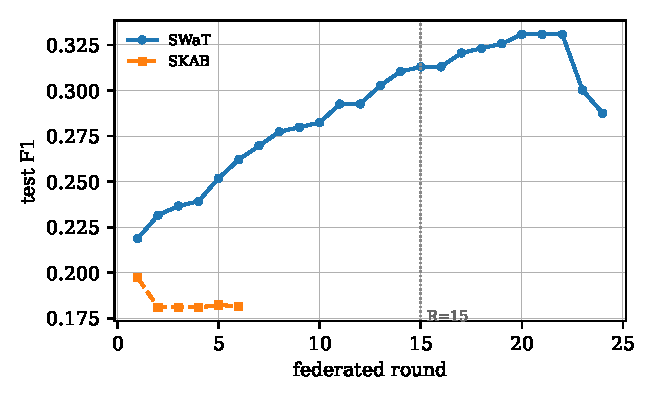
\includegraphics[width=0.6\linewidth]{figs/fig_convergence}
\caption{Per-round test F1 (full data, $\varepsilon{=}2$). SKAB converges by round~$6$;
SWaT is near-plateau by round~$15$ (dotted line). Source:
\texttt{convergence\_curve.json}.}\label{fig:conv}
\end{figure}

\section{Software environment}\label{supp:env}
All experiments were run on a single workstation (Intel Core i5-1335U CPU, 16\,GB RAM,
no GPU) with the following pinned versions (also in the
released \texttt{requirements.txt}): Python~3.13, PyTorch~2.12.0, Opacus~1.6.0,
scikit-learn~1.7.2, NumPy~2.2.0, SciPy~1.16.2, pyarrow~24.0.0, faiss-cpu~1.13.0,
matplotlib~3.10.6. Datasets are loaded from cached NumPy archives to avoid a
native library load-order conflict (the parquet reader must be imported before the
deep-learning stack). Every reported number is regenerated by the corresponding
script and written to a JSON file under \texttt{results/}; no value is hand-entered.

\bibliographystyle{sn-mathphys-num}
\bibliography{references}
\end{document}
